%!TEX root = ../dokumentation.tex


\chapter{Sudoku}
Nachdem in der Einleitung schon kurz auf das Spielfeld eines Sudokus und die Regeln eingegangen wurde, werden beides in diesem Kapitel noch einmal ausführlicher behandelt. Es wird auch auf Elemente des Spielfelds eingegangen, die relevant sind für die Strategien und wie das Spielfeld in dem Programm aufgebaut ist. 


\section{Spielfeld Aufteilung}
Das Spielfeld auf dem ein Sudoku gespielt wird besteht aus einem 9x9 Gitter und damit aus 81 einzelnen Zellen. Diese Gitter lässt sich nochmal aufteilen mit drei verschiedenen \textbf{Units}. Jede \textbf{Unit} besteht immer aus 9 Zellen. Damit kann ein Sudoku also nochmal in 27 verschiedene Zellen aufgeteilt werden. Wie diese \text{Units} 

\subsection{Zeile}
Eine Zeile in einem Sudokuspielfeld sind Zellen die horizontal zueinander ausgerichtet sind. In der Abbildung \ref{fig:SudokugitterZeile} wurde die oberste Zeile beispielhaft markiert.
\begin{figure}[htbp]
	\centering
	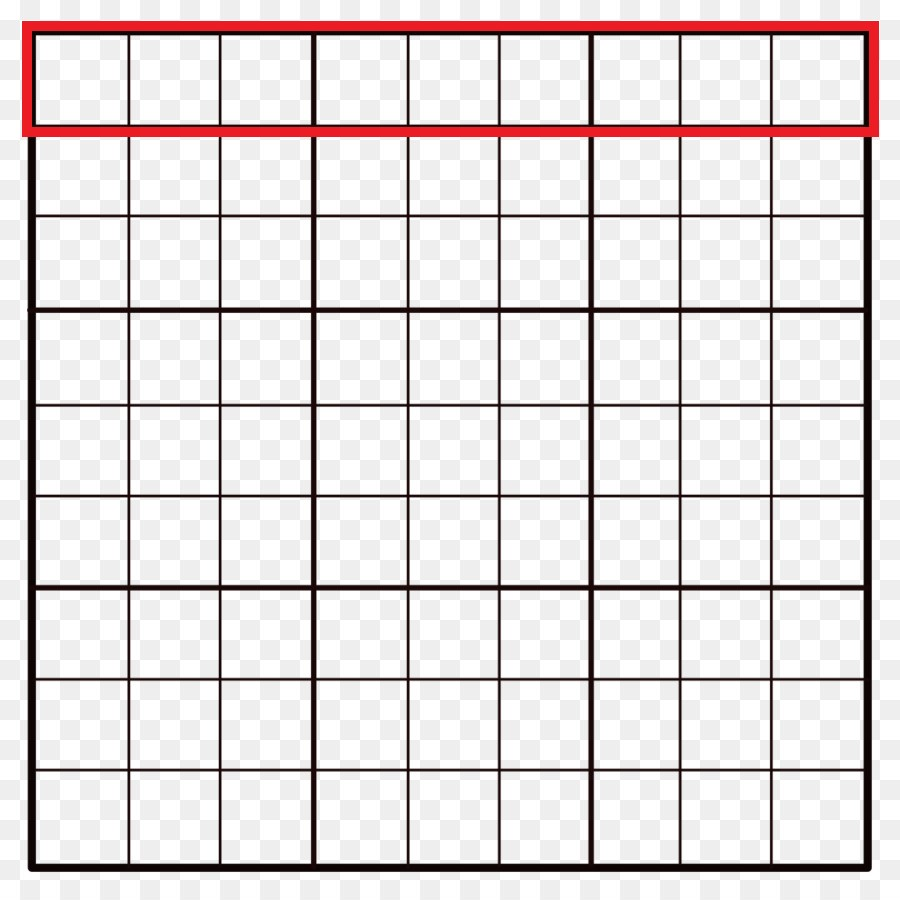
\includegraphics[width=0.3\textwidth]{images/sudokugitterZeile.jpg}
	\caption{Darstellung des Sudokugitters mit der Markierung einer Zeile}
	\label{fig:SudokugitterZeile}
\end{figure}

\subsection{Spalte}
Analog zu einer Reihe sind Spalten Zellen die vertikal zueinander ausgerichtet sind. In der Abbildung \ref{fig:SudokugitterSpalte} wurde beispielhaft eine Spalte markiert.
\begin{figure}[htbp]
	\centering
	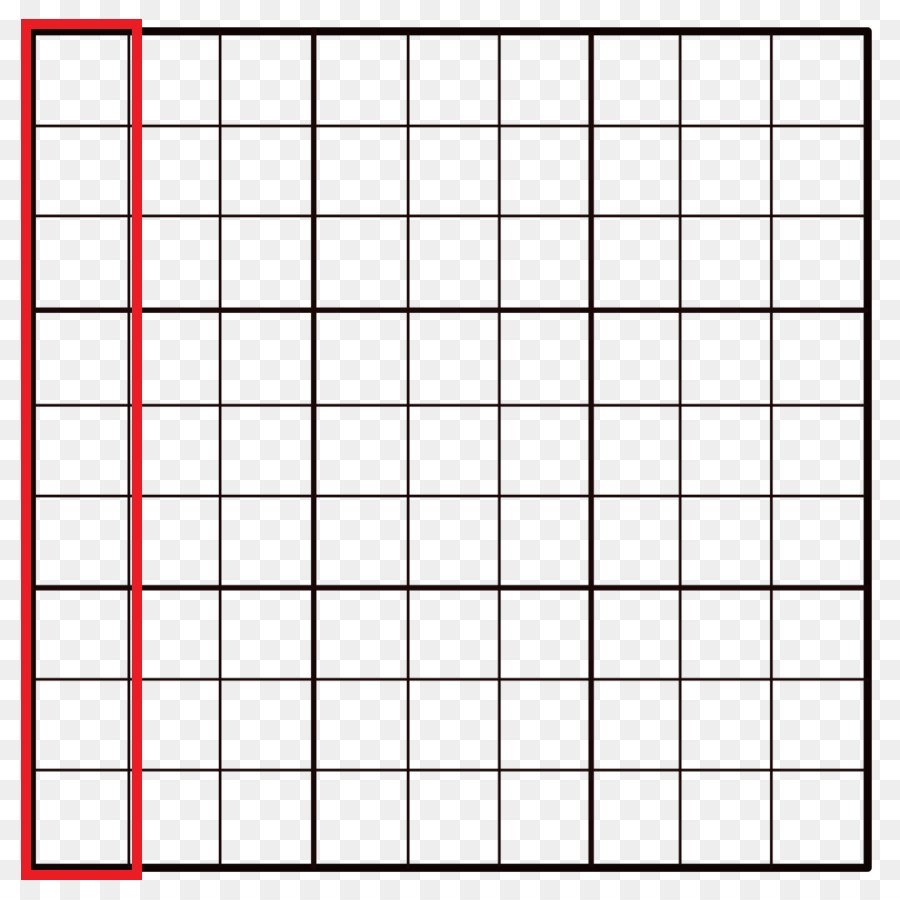
\includegraphics[width=0.3\textwidth]{images/sudokugitterSpalte.jpg}
	\caption{Darstellung des Sudokugitters mit der Markierung einer Spalte}
	\label{fig:SudokugitterSpalte}
\end{figure}

\subsection{Box/Block}
Boxen bestehen aus 3x3 Zellen. Boxen können aber nicht einfach so an jeder beliebigen Stelle eines Sudokus erstellt werden. Der rechte untere Wert einer Box muss sowohl in der x-Achse durch drei teilbar sein, wie in der y-Achse. In der Abbildung \ref{fig:SudokugitterBox} wurde eine Box markiert. Die markierten Zellen können kein Teil einer weiteren Box mehr sein. Wie in der Abbildung \ref{fig:SudokugitterBox} zu erkennen ist sind die Boxen auch im Frontend durch dickere Linien voneinander abgegrenzt. 
\begin{figure}[htbp]
	\centering
	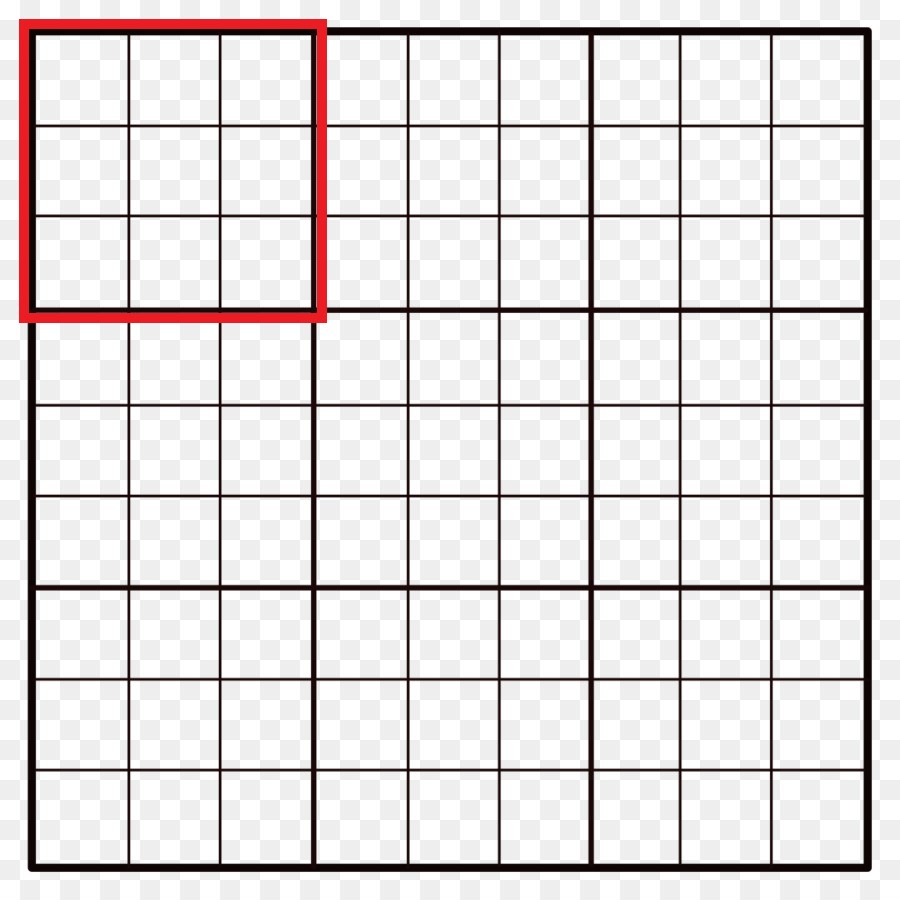
\includegraphics[width=0.3\textwidth]{images/sudokugitterBox.jpg}
	\caption{Darstellung des Sudokugitters mit der Aufteilung in 9 Boxen}
	\label{fig:SudokugitterBox}
\end{figure}

\section{Regeln}
Für die Regeln ergeben sich einfache Bedingungen wenn man die Aufteilung des Spielfeldes kennt. In jeder Zeile dürfen die Zahlen eins bis neun nur einmal vorkommen. Genau dieselbe Bedingung gibt es für eine Spalte und für einen Block.

Am Ende kommen die Zahlen eins bis neun also jeweils neunmal auf dem gesamten Sudokugitter vor und in jedem Block, jeder Zeile und jeder Zeile genau einmal.

Damit man das Sudokugitter ausfüllen kann sind zu Spielbeginn einige Ziffern vorgegeben. Mithilfe dieser Ziffern ist es möglich mit den gerade erklärten Regeln das ganze Sudokugitter zu füllen. 

\section{Strategie}
Um ein Sudoku zu lösen können verschiedene Strategien umgesetzt werden. Das Ziel einer Strategie ist es hierbei eine passende Zahl in das Sudoku einzufügen oder mögliche Kandidaten zu eliminieren. Es gibt zwei Strategien um direkt Zahlen einfügen zu können, nämlich den Hidden Single und den Naked Single. Beide Strategien können oft intuitiv und ohne eine große Erklärung anwenden. Weitere leichte Strategien wie ein Hidden Double oder ein Naked Double können mithilfe der Kandidaten-Notation gefunden und angewendet werden.

Insgesamt gibt es über 20 Strategien die bei schweren Sudokus angewendet werden können. Zum Teil sind die Strategien für das menschliche Auge schwer zu entdecken und auch schwer zu erläutern. Wichtig bei diesen schweren Strategien ist eine gewissenhafte Ausführung der Kandidaten-Notation.
\todo{https://www.thinkgym.de/r\%C3\%A4tselarten/sudoku/l\%C3\%B6sungsstrategien-1/}
\subsection{Lösungshilfen: Kandidaten-Notation}
Kandidaten sind Zahlen in einer Zelle des Sudokugitters, die die Möglichkeit besitzen in diese Zelle eingetragen zu werden. Das Problem liegt aber dabei, dass mehrere Zahlen in diese Zelle können, weil es noch nicht genügend andere feste Zahlen gibt, die bereits eingetragen wurden. Wenn man dabei jede Zelle einzeln betrachtet geben die Kandidaten keinen weiteren Nutzen. Jedoch, wenn die Kandidaten mehrerer Zellen in Bezug zueinander angeschaut werden, lassen sich Zusammenhänge erkennen. Aufgrund dieser Erkenntnisse wurden weitere Strategien entwickelt. 

Sobald eine Zahl mittels des Hidden Single oder des Naked Single eingetragen wird, müssen die Kandidaten aktualisiert werden. Es besteht die Möglichkeit, dass man einige Kandidaten die denselben Wert haben wie die neu eingetragene Zahl und in Zellen stehen, die eine Verbindung über eine Reihe, Spalte oder einen Block haben zu der Zelle in der die Zahl eingetragen wurde, herausgestrichen werden können. 
